\documentclass{article} % For LaTeX2e
\usepackage{nips12submit_e,times}

\usepackage{color}
\usepackage{algpseudocode}
\usepackage{algorithm}
\usepackage{listings}
\usepackage{graphicx}
\usepackage{subcaption}
\usepackage{caption}
\usepackage{float}

\definecolor{javared}{rgb}{0.6,0,0} % for strings
\definecolor{javagreen}{rgb}{0.25,0.5,0.35} % comments
\definecolor{javapurple}{rgb}{0.5,0,0.35} % keywords
\definecolor{javadocblue}{rgb}{0.25,0.35,0.75} % javadoc
% "define" Scala
\lstdefinelanguage{scala}{morekeywords={class,object,trait,extends,with,new,if,while,for,def,val,var,this},
otherkeywords={->,=>},
sensitive=true,
morecomment=[l]{//},
morecomment=[s]{/*}{*/},
morestring=[b]"}
% Default settings for code listings
\lstset{frame=tb,language=scala,aboveskip=3mm,belowskip=3mm,showstringspaces=false,columns=flexible,basicstyle={\small\ttfamily},
keywordstyle=\color{javapurple}\bfseries,
stringstyle=\color{javared},
commentstyle=\color{javagreen},
morecomment=[s][\color{javadocblue}]{/**}{*/}}
%\documentstyle[nips12submit_09,times,art10]{article} % For LaTeX 2.09


\title{A Comparison of Parallel Algorithms:\\ {\Large Hogwild!, Shotgun and Distributed Averaging}}

\author{
David A. Leen \\
Department of Applied Mathematics\\
University of Washington \\
\texttt{dleen@uw.edu} \\
\And
Brian D. Walker \\
Department of Computer Science \& Engineering \\
University of Washington \\
\texttt{walker7734@gmail.com} \\
}

% The \author macro works with any number of authors. There are two commands
% used to separate the names and addresses of multiple authors: \And and \AND.
%
% Using \And between authors leaves it to \LaTeX{} to determine where to break
% the lines. Using \AND forces a linebreak at that point. So, if \LaTeX{}
% puts 3 of 4 authors names on the first line, and the last on the second
% line, try using \AND instead of \And before the third author name.

\newcommand{\fix}{\marginpar{FIX}}
\newcommand{\new}{\marginpar{NEW}}

\nipsfinalcopy % Uncomment for camera-ready version

\begin{document}
\maketitle

\begin{abstract}
We implemented the Hogwild! algorithm and demonstrated an approximately linear speedup over the
sequential stochastic gradient descent (SGD) algorithm.  We used the click prediction dataset and its sparse search token features to test the algorithms. We implement and demonstrate the close to optimal speedup of the Distributed Averaging method. Several strategies are detailed for dealing with mixed-sparsity data i.e. data that has both sparse and dense components. We implement a potentially novel combination of Hogwild!~and Distributed Averaging. We demonstrate the favorable trade-off between speedup and test error that this method gives on mixed-sparsity data. We finally test these algorithms on some synthetic data derived from the click prediction data set, where the number of dense user features and sparse tokens is increased.
\end{abstract}

\section{Introduction}
We study three parallel algorithms: Hogwild! \cite{niu2011hogwild}, Shotgun \cite{bradley2011parallel} and distributed averaging \cite{zhang2012comunication}. Each approaches a similar problem in a distinct manner. Hogwild! and distributed averaging parallelize stochastic gradient descent (SGD) over samples, whereas Shotgun tackles the orthogonal problem of parallelizing $L_1$-regularized models over the features.

Hogwild!~is just one particular realization of parallel SGD \cite{niu2011hogwild, zinkevich2010parallelized}. The algorithm is intended for problems on the order of several terabytes of data. It can be run quite effectively on inexpensive multi-core systems taking advantage of the low latency and high throughput of the data being stored in RAM or a RAID disk setup close to the processors. In these systems the bottlenecks arise from synchronizing and locking operations on the threads reading and writing shared memory. Regularization can also be applied in parallel settings \cite{langford2009slow, agarwal2011distributed}.

MapReduce in contrast deals with hundreds and thousands of terabytes of data but is not well suited for online, iterative algorithms like SGD. MapReduce suffers from low throughputs due to fault tolerance and redundancy. Distributed averaging is a simple version of a distributed optimization algorithm \cite{dekel2012optimal, agarwal2011distributed}. The method distributes the data samples evenly in group to some number of machines. Each machine performs a separate minimization of each group independently of one another. The estimates of the weights from each group are then averaged hence the name.

Shotgun provides a parallel solution to the high-dimensional problem with a large number of features using $L_1$-regularization \cite{ng2004feature}. In cases like this the dimensionality of the problem often dwarfs the number of samples. Once again the method involves taking a sequential algorithm, coordinate descent and simply parallelizes it, this time over features. The algorithm makes the coordinate updates in parallel to provide a speedup.

We study these algorithms in the context of the click prediction dataset. We first briefly discuss the algorithms, the challenges associated with parallel programming, then specific challenges associated with the click prediction dataset. Finally we present our results and our ``replicate'' strategy for mixed-sparsity data.

\section{Method}
The weight vector $w$ for logistic regression is updated according to the usual SGD equation:
\begin{equation}
w_i^{t+1} \leftarrow w_i^t + \eta \bigg[y^t - \frac{\exp{(w^t \cdot x^t)}}{1 + \exp{(w^t \cdot x^t)}} \bigg]x_i^t.
\end{equation}

%\subsection{Proof of concept}
%The minimal example demonstrating the Hogwild! concept in practice for a simple mapping is (in Scala for brevity):
%\begin{lstlisting}
%val weights = collection.mutable.Map[Int, Double]() // create a mapping
%for (i <- data.keys) weights.put(i, 0.0) // initialize key values to 0.0
%for (k <- samples.par, i <- feature.keys) weights(i) += gradient // update
%\end{lstlisting}
%This parallel version of SGD (using the \verb+.par+ method) produces non-deterministic values for the weights as expected. This is due to a race condition caused by threads overwriting one another. The Hogwild! algorithm relies on the sparsity of the data to ensure that updates do not operate simultaneously on the same keys. It relies on the same sparsity to parallelize the sequential algorithm.

\subsection{Algorithm}

\begin{algorithm}
  \caption{Hogwild! update step for a single processor}

  \begin{algorithmic}
  \Loop
  \State Randomly permute data
  \State Read current state of features $x^t$
  \For {i in $x^t$.keys}
  \State $w^{t+1}_i \leftarrow w_i^t - \eta x_i^t \nabla L(\mathbf{w}, \mathbf{x}, \mathbf{y})$
  \EndFor
  \EndLoop
  \end{algorithmic}
  \label{alg1}
\end{algorithm}

The component wise addition of elements from the weight vector is assumed to be atomic. In practice floats are not atomic and require extra care. See section \ref{gen_inst}.

\section{Challenges and issues}
\label{gen_inst}
\subsection{Parallel and concurrent programming}
Parallel programming is hard. The Hogwild!~solution is to ignore all the major issues associated with parallelism. The Hogwild!~paper discusses a compromise between full synchronization and no locking at all which they call AIG. AIG puts a lock on only the elements that are being updated inside the for loop in algorithm \ref{alg1}. This is essentially what ConcurrentHashMap in Java does. It often can be difficult to determine which regime we are operating in without resorting to a closer-to-the-hardware language like C.

Distributed Averaging takes the opposite approach avoiding the issues of parallelism altogether. It turns the problem into a data parallel one by dividing the data into a number of chunks, one per machine or processor and running SGD in parallel on each one independent of the others. The weights are then averaged. 

\subsection{Storing data in memory}
The Hogwild!~algorithm relies on extremely fast throughput of data from memory or disk. Reading from disk is not fast enough to supply data as needed by a 4-6 core machine. This could be possible with a RAID setup but at the time this was not available. The Hogwild!~paper uses sophisticated caching and memory management to process terabyte sized data on a single machine.

Our current solution is to load and parse all the data into RAM. 8--16GB of RAM is fairly standard these days, which is sufficient for the click prediction set, but it is not enough for terabyte data sets. We need to investigate how to break data sets into manageable chunks while still sampling uniformly as needed by the algorithms. 

\subsection{Non-sparse data}
An immediate issue was whether Hogwild! can work efficiently on data with sparse and non-sparse components? The click prediction data has several dense values including age and gender. They are updated on every iteration. The tokens however are very sparse. Can we apply the Hogwild! algorithm in this case without ignoring the dense data? This issue is answered in the next section.

\section{Mixed-sparsity data}
The click prediction data provides an interesting scenario in which to test Hogwild! The click prediction dataset is comprised of user features and sparse tokens. We call this combination of sparse and non-sparse data ``mixed-sparsity''. We initially pretend the data is sparse and run Hogwild!~ before discussing strategies for improving the error while maintaining the speedup from the extra processors.

As expected not dealing with the non-sparse data allowed for the expected speedup but as more processor cores were introduced the error spiked as there were more data collisions with the non-sparse features. We took this as a good opportunity to explore methods to handle the non-sparse data and still obtain a substantial speedup from the Hogwild! algorithm.  We explored five methods to handle the non-sparse features.

\subsection{Strategies for mixed-sparsity data}
We outline several strategies that we implement and test on the click prediction dataset:
\begin{enumerate}
\item {\em Normal}: this strategy simply treats all of the data as sparse regardless as to whether it truly is.  Therefore, we run Hogwild!~with absolutely no locking on any of the data features and let data collisions occur without any attempt to prevent them. This is less of a strategy for dealing with non-sparse data as it is a baseline with which we can compare our other strategies. 
\item {\em Locking}: the most obvious strategy is to lock the data to prevent data collisions.  However, the whole point of the Hogwild!~algorithm is to gain a near linear speedup by not using locking. The introduction of locks forces a portion of the algorithm to run sequentially and thus has the potential to kill our speedup. Since only a small portion of our data is non-sparse we only lock during the update of these non-sparse features and allow the remaining sparse data to continue lock-free. 
\item {\em Random}: this strategy attempts to prevent data collisions by giving all the threads an equal probability to update the non-sparse weights. To implement this strategy we use a random number generator that produces a number from zero to the number of current threads. If that threads generated number is zero then it updates the non-sparse data. This allows the data to be updated once, on average, for each iteration.  Data collisions are still allowed to occur and no locking is done. 
\item {\em Single thread}: to completely prevent any chance of data collisions this strategy randomly chooses one thread at the start of the algorithm to be the only thread to update the non-sparse weights. This strategy allows us to remain lock-free and have a zero chance of data collisions. This comes at the cost of updating the non-sparse data less frequently.
\item {\em Replicate}: this strategy attempts to eliminate the problem of data collisions while still allowing the non-sparse weights to be based on more information than is provided by just a single thread. Instead of assigning a single thread or randomizing to determine which thread can update the non-sparse data, we allow all of them to update their own copies of the non-sparse data.  Each thread is given its own copy and updates the non-sparse data independently and thus without locks.  The sparse data still remains in shared memory and the updates to these features remains unchanged from the original Hogwild!~algorithm. When the algorithm has completed we then average the non-sparse data from each of the threads back into shared memory. This allows us to tally the information from all of the threads with the hope of achieving more accurate weights. 
\end{enumerate}

\section{Results}
Initial results ranging from one to four CPU cores (figure \ref{res}). During each run the same number of updates over the data occurs with the workload evenly distributed across each core. We fall slightly short of the optimal speedup of four, figure \ref{res}(a). The Hogwild! algorithm has a slightly worse RMSE as expected, figure \ref{res}(b).
\begin{figure}[H]
\centering
\begin{subfigure}{0.35\textwidth}
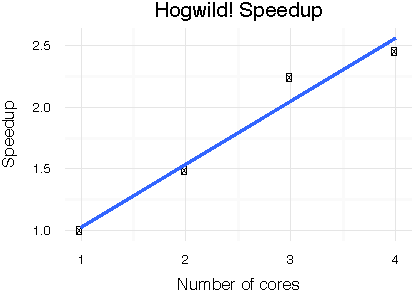
\includegraphics[width=\textwidth]{./speedup.pdf}
\end{subfigure}
\centering
\begin{subfigure}{0.35\textwidth}
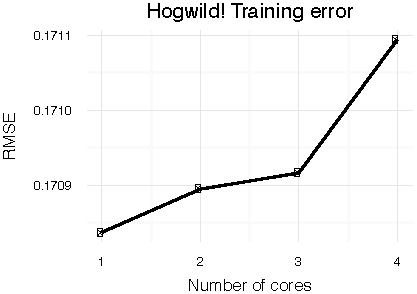
\includegraphics[width=\textwidth]{./error.pdf}
\end{subfigure}
\caption{(a) The observed speedup from experiment. The speedup with four processors is approximately 2.55.~(b) The observed root mean squared error growth with number of cores from experiment.}
\label{res}
\end{figure}

Distributed averaging (figure \ref{dist_avg}) achieves near optimal speedup as each processor runs independently of one another and do not need to communicate. The error suffers as each processor only trains on a fraction of the data.

\begin{figure}[H]
\centering
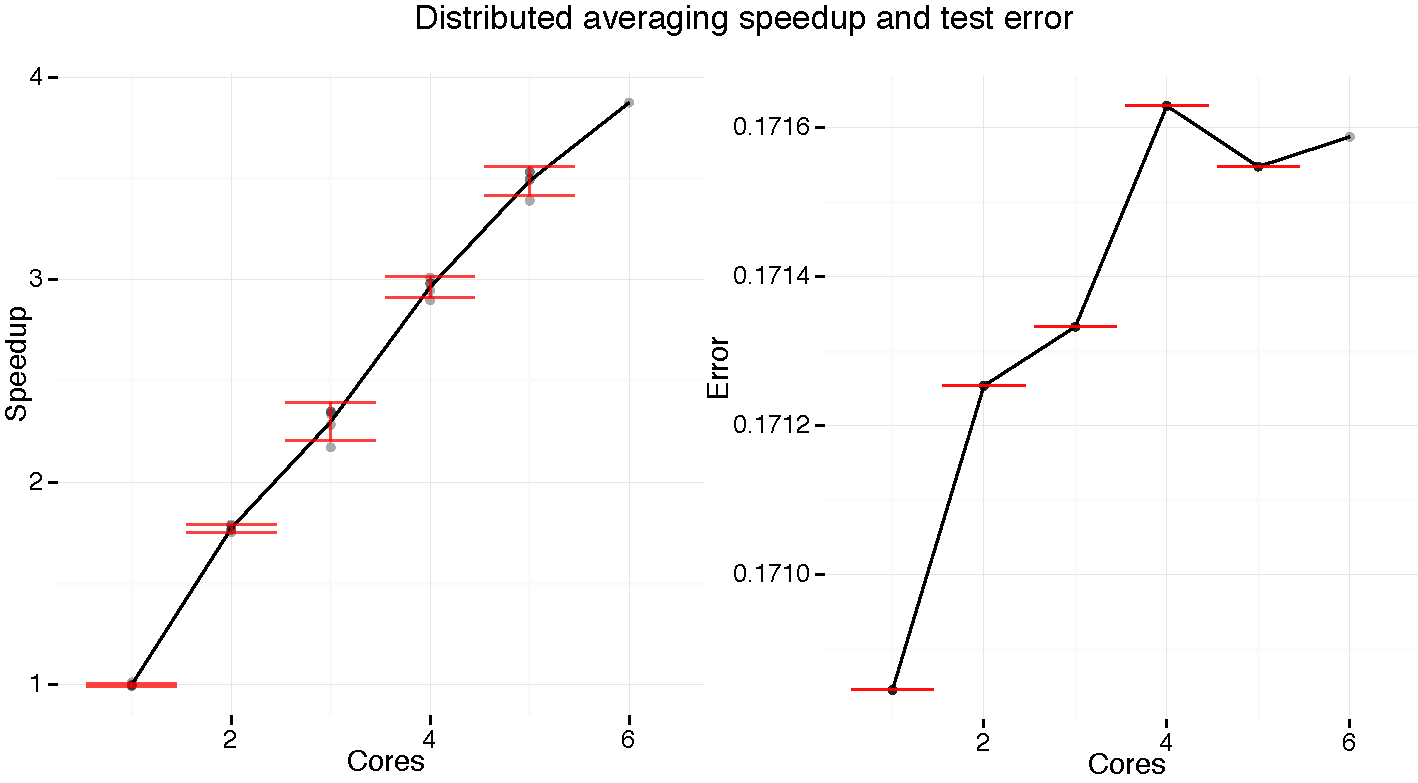
\includegraphics[width=0.8\textwidth]{../../dist_avg.pdf}
\caption{Distributed averaging achieves nearly optimal speedup as there is no communication overhead between the processors. The SGD is computed independently for each processor. The error increases drastically as the data is split more and more and each processor trains the weights on less and less data.}
\label{dist_avg}
\end{figure}

We now discuss the results of our strategies for dealing with mixed-sparsity data. Figure \ref{speedup_all} displays the results of our numerical experiments. The main result is that the replication technique out-performs everything else in terms of speedup-error tradeoff. It combines the the speedup and advantages of Hogwild!~with the batch processing of distributed averaging for the dense data components.

\begin{figure}[H]
\centering
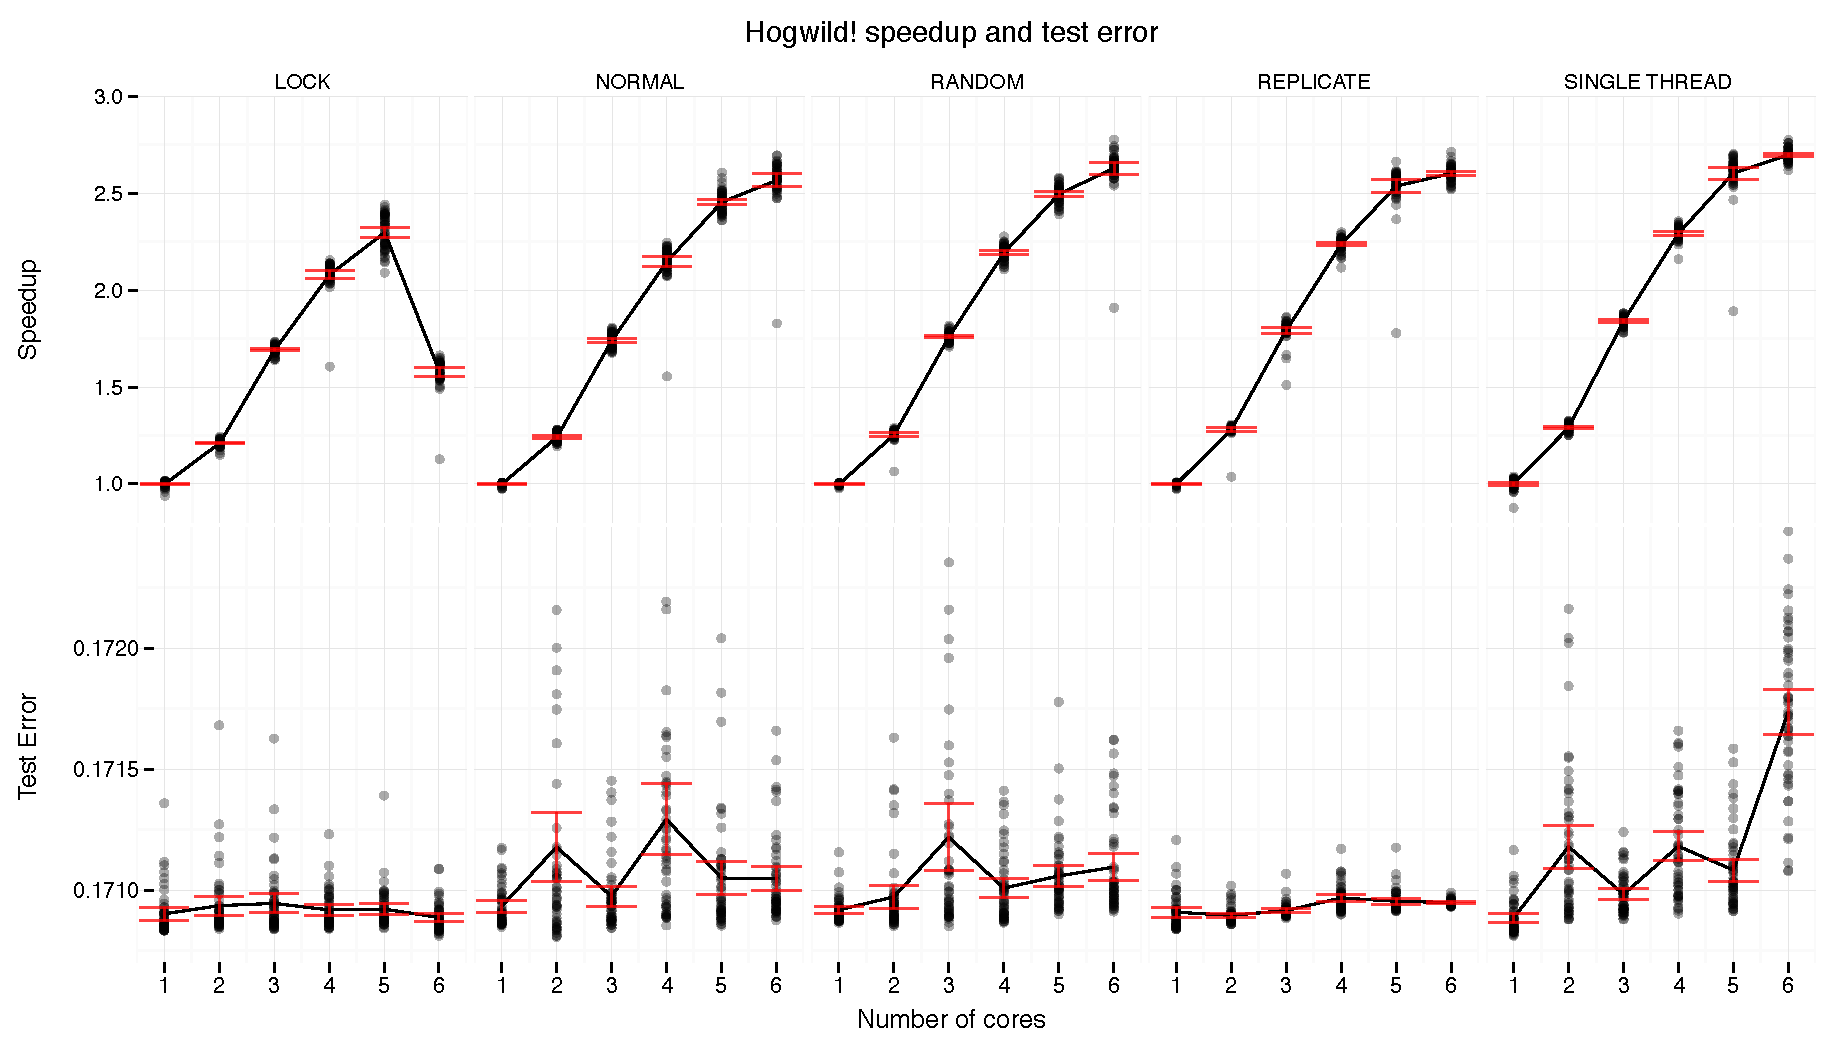
\includegraphics[width=\textwidth]{../../speedup_errors_complete.pdf}
\caption{A comparison of our strategies for dealing with mixed-sparsity data. Lock suffers greatly in speedup as the number of processors increases from one to six. This is because of processors waiting for locked resources. The test error is constant in the number of processors and is consistently the best among all the algorithms. Normal and random have similar speedup performances and have high variances in the errors which are larger than the locked and replicate case. Random does as well as treating the data as sparse and achieves better errors. Single thread performs the worst as it trains the weights on only a fraction of the data. Replicate is our novel attempt at the mixed-sparsity problem. The speedup is as good as the other cases and the error is almost as good as the locking case. This is both a surprising and promising result.}
\label{speedup_all}
\end{figure}

We generate synthetic data (figure \ref{speedup_syn}) derived from the click prediction data by increasing the size of the dense user features and increasing the number of sparse features. This causes the locking algorithm even more problems. The other algorithms see an increase in speedup as the processors spend relatively more time calculating the gradient compared to communication and memory overhead.

\begin{figure}[htb]
\centering
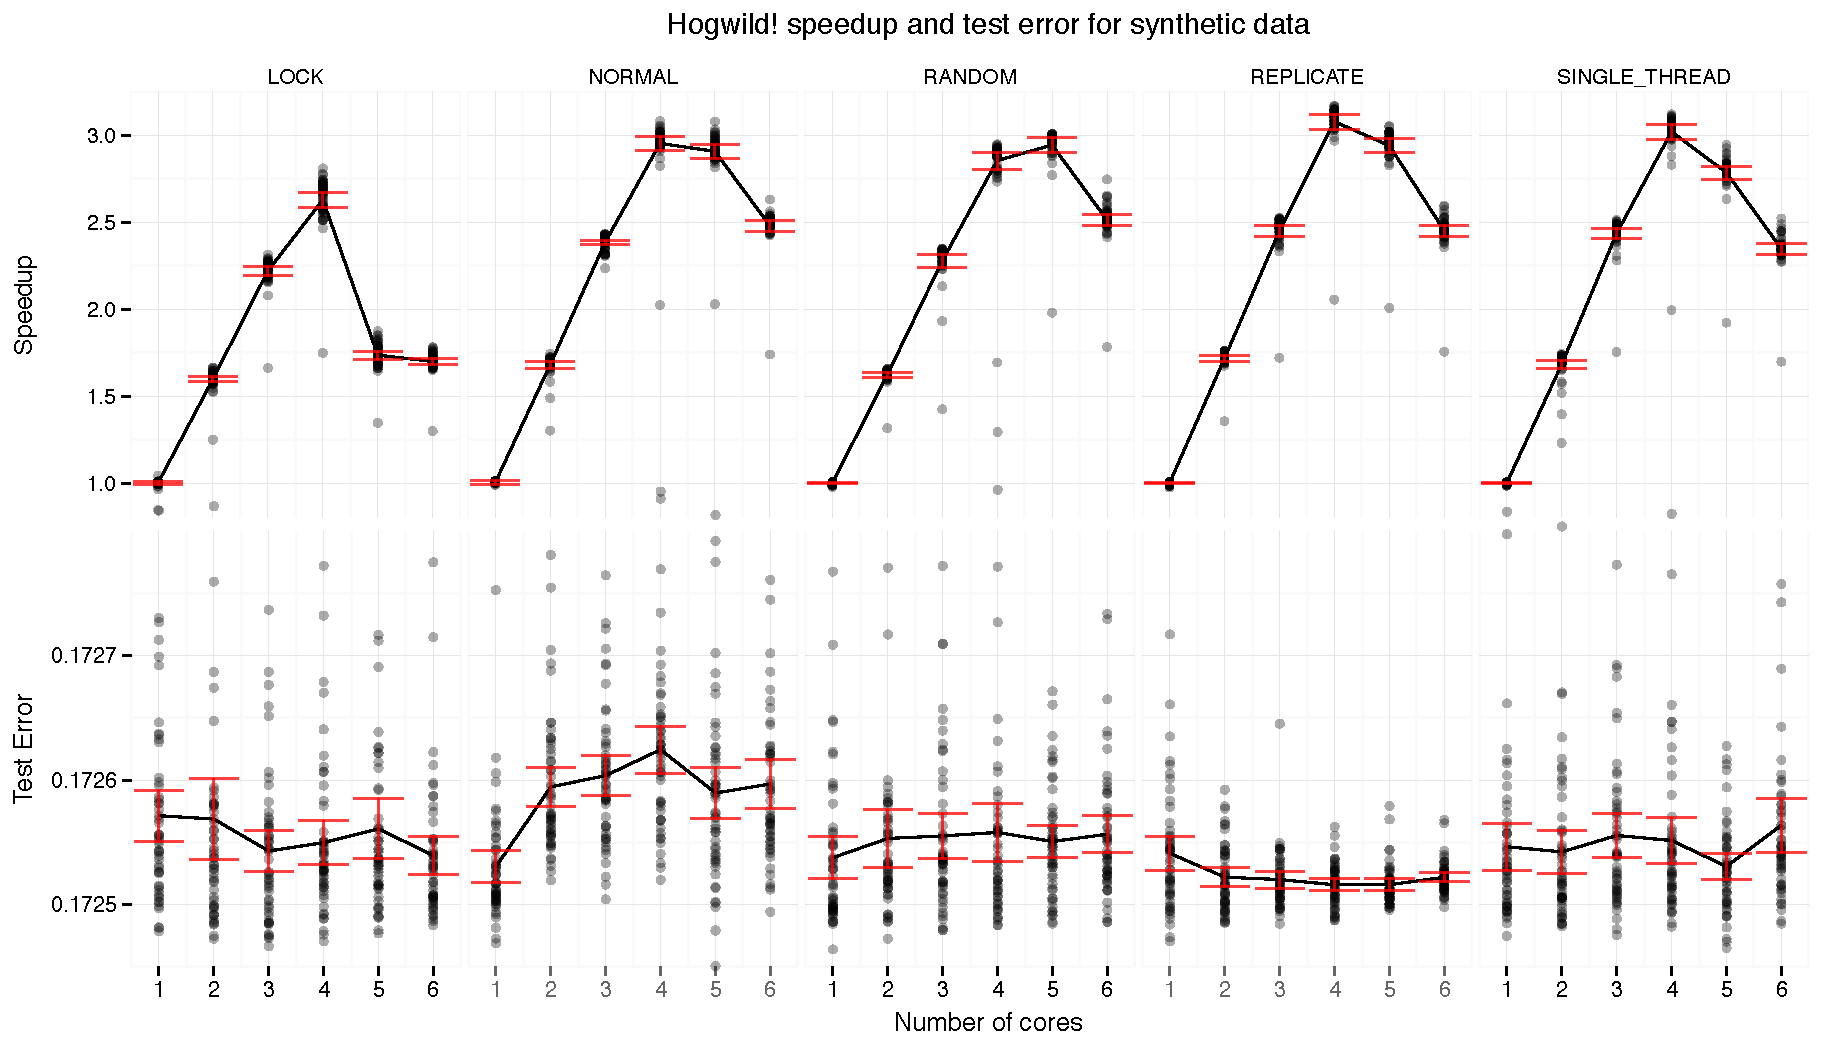
\includegraphics[width=\textwidth]{../../speedup_errors_complete_syn.pdf}
\caption{Synthetic data is created from the click prediction data by doubling the number of user features from five to ten and increasing the number of sparse features per sample to 50. This increases the amount of work for each processor and hence we see a greater speedup. The lock strategy suffers the most due to scheduling of the greater workload. Replicate amazingly has the best error and greatest speedup. The test error variance is also very small compared to the others. This was a surprisingly good result. Random and normal suffer from the worst errors as expected.}
\label{speedup_syn}
\end{figure}

Plotting the test error against the wall time (figure \ref{wall time}) clearly demonstrates the strengths of the replicate algorithm.

\begin{figure}[htb]
\centering
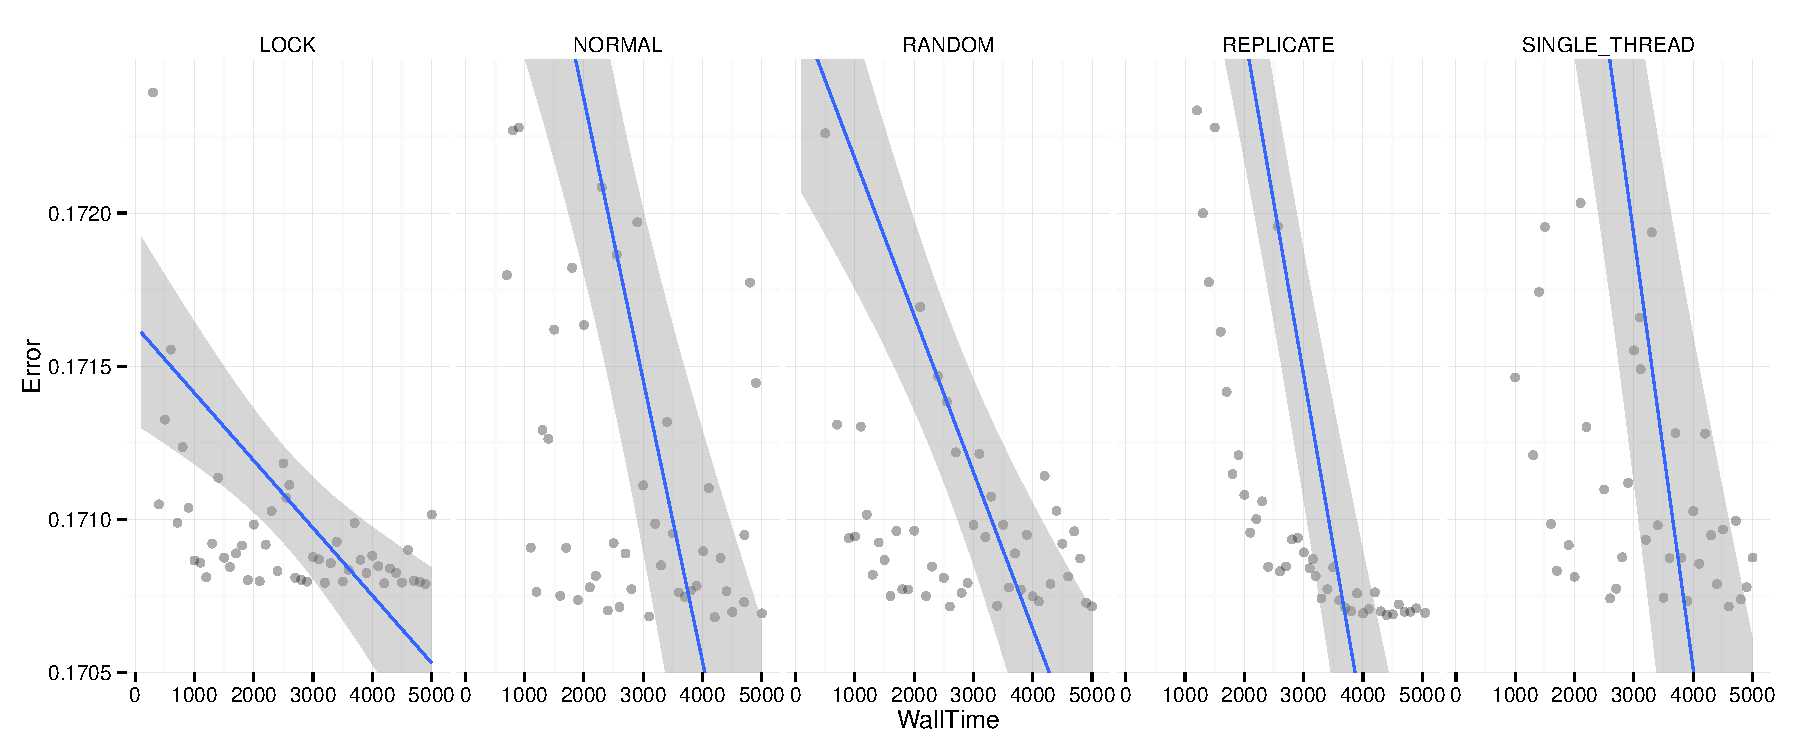
\includegraphics[width=\textwidth]{../../walltime_6.pdf}
\caption{The test error as a function of wall time. Locking achieves the best error among all the algorithms as expected. This suffers greatly in speedup performance however. Normal is quite noisy as we are treating the data as sparse and the processors will frequently overwrite one another. Random has the worst error out of all of them. Replicate is again surprising as it performs almost as well. Single thread performs about as well as normal.}
\label{walltime}
\end{figure}


\newpage
\section{Further work}
Further work involves a theoretical analysis of the error bounds of our replicate algorithm. 

\newpage
\subsubsection*{References}
\begingroup
\renewcommand{\section}[2]{}%
\bibliographystyle{unsrt}
\bibliography{references}
\endgroup
\end{document}
